\documentclass{article}
\usepackage[utf8]{inputenc}
\usepackage{graphicx}
\usepackage{amsmath}
\usepackage{amssymb}
\usepackage{subfig}
\usepackage{listings}
\usepackage{algorithm}
\usepackage{algorithmic}
\usepackage{caption}
\usepackage{url}

\title{Machine Learning with Graphs:\\ Homework 5 - Graph Neural Networks and Knowledge Graphs\\ Due: 04/28}
\author{}
\date{Spring 2026}

\begin{document}

\maketitle

Reminder: You can choose to solve problem 2 or 3.

\section*{Problem 1 (conceptual)}

\paragraph{a)} In class, we described GCNs from the basic idea of graph filters up to the much simpler notion of graph convolution that is applied in practice. Give an example of how the simplifications applied might prevent an single-layer GCNs from solving problems that the original formulation of learnable spectral filters could solve.

\paragraph{b)} Consider the graph from Figure \ref{fig::p1b}, where each node has a unique feature represented as a one-hot encoding. Show the computations of an single-layer GCN for the graph in the figure. Describe the total computation cost in terms of number of operations. Discuss how the computation could be made more efficient in this specific example.

\begin{figure}
\centering
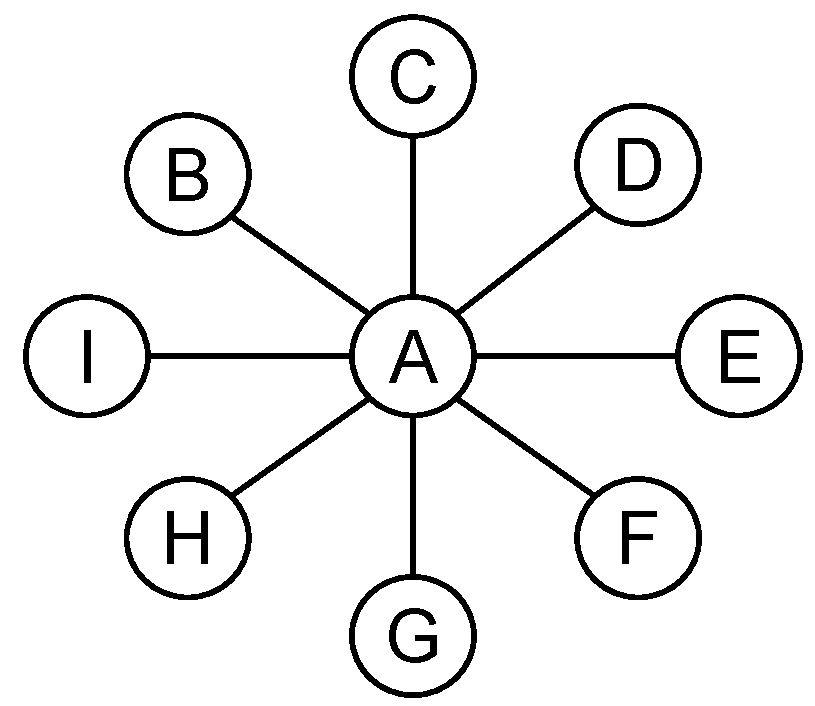
\includegraphics[keepaspectratio,width=0.4\textwidth]{figures/hw5-p1b}
\caption{Problem 1b. \label{fig::p1b}}
\end{figure}

\paragraph{c)} Besides the types of KG relations discussed in class, consider cyclic relations in the form $(e_1,r,e_2), (e_2,r,e_3), \ldots (e_k,r,e_1)$. Provide a real example of a relation that can have a cyclic pattern as described. Briefly discuss whether TransE and TransR can capture cyclic relations and why.

\paragraph{d)} We showed in class that TransR embeddings can capture each relation type independently. However, we have not discussed whether satisfying one relation type can hurt another. Is this possible? If so, provide an example where satisfying one relation type adversely affects the representation of another.

\section*{Problem 2 (optional, analytical)}

There is a growing interest in applying GNNs to solve graph combinatorial problems. Here, we will consider whether GNNs can theoretically solve decision (YES/NO) problems on graphs.

a) Provide an example of an NP-complete decision problem and show that a 1-WL-powerful GNN cannot solve the problem.

b) Someone might claim that a 1-WL-powerful GNN can always solve a decision problem for which there is a poly-time algorithm. Discuss whether that is true or false, either with a proof or an example.

\section*{Problem 3 (optional, coding)}

In class, we have discussed types of relations in KGs and whether different KG embedding methods are able to capture them or not. In this question, we will investigate KG capabilities empirically. For that, you will need a library that implements KG embedding methods, such as Pytorch Geometric (PyG).\footnote{\url{https://pytorch-geometric.readthedocs.io/en/latest/index.html}}

\paragraph{a)} Use your knowledge of TransE limitations to create a simple synthetic graph where TransE will achieve poor performance on KG completion and provide an experiment evaluating the performance of TransE for your example. Note that the cause of the poor performance should be explained by the inability of TransE to capture certain relationship patterns. Show how a more powerful KG embedding model performs better for your example.

\paragraph{b)} Select two types of relations that DistMult is not able to capture and estimate how often such types of relations occur in the FB15k-237 dataset.\footnote{\url{https://www.kaggle.com/datasets/latebloomer/fb15k-237}} Provide some quantitative analysis of how the frequency of the two types of relations you chose will impact the performance of DistMult for KG completion using FB15k-237


\end{document}
